\documentclass[11pt, oneside]{article}   	% use "amsart" instead of "article" for AMSLaTeX format
\usepackage{geometry}                		% See geometry.pdf to learn the layout options. There are lots.
\geometry{letterpaper}                   		% ... or a4paper or a5paper or ... 
%\geometry{landscape}                		% Activate for rotated page geometry
%\usepackage[parfill]{parskip}    		% Activate to begin paragraphs with an empty line rather than an indent
\usepackage{graphicx}				% Use pdf, png, jpg, or eps§ with pdflatex; use eps in DVI mode
\usepackage{ragged2e}						% TeX will automatically convert eps --> pdf in pdflatex		
\usepackage{amssymb}
\usepackage{amsmath}
\usepackage{float}
\usepackage{listings}
\lstset{language=R,
    basicstyle=\small\ttfamily,
    stringstyle=\color{DarkGreen},
    otherkeywords={0,1,2,3,4,5,6,7,8,9},
    morekeywords={TRUE,FALSE},
    deletekeywords={data,frame,length,as,character},
    keywordstyle=\color{blue},
    commentstyle=\color{DarkGreen},
     %frame=single, % adds a frame around the code
     backgroundcolor=\color{lightgray},
}
\usepackage[svgnames]{xcolor}
%SetFonts

%SetFonts


\title{Assignment 9}
\author{Yapi Donatien Achou}
%\date{}							% Activate to display a given date or no date

\begin{document}
\maketitle
\section{Problem 9.1}
\subsection{Part a: Loading and plotting data}
\begin{figure}[H] %  figure placement: here, top, bottom, or page
   \centering
   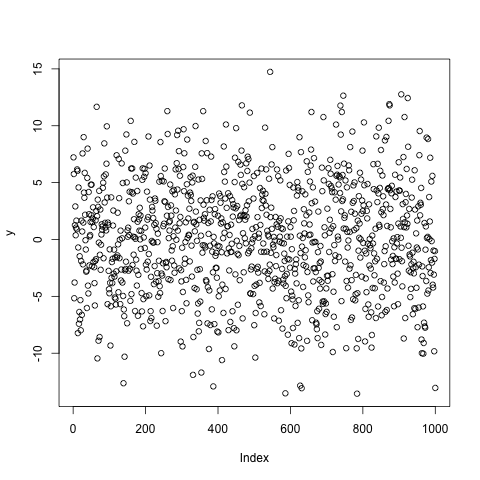
\includegraphics[width=4in]{maq} 
   \caption{Simulated MA(q) process with gaussian noise}
   \label{fig:example}
\end{figure}
%%%%%%%%%%%%%%%%%%%%%%%%%%%%%%%%%%%%%%%%%%%%%%%%%%%%%%%%%%%%

\subsection{Part b: simulate MA(k)}
The AIC (Akaikes Information Criteria) and BIC (Bayesian Information Criteria) are penalised-likelihood information criteria \cite{ziak, petter} used for model selection.  A model with too few parameters can have a large bias while a model with too many parameters can promote overfitting by not generalising enough. Furtheremore, the mean square error of the forecasts model depends on the white noise variance of the fitted model and on the error arising from the estimation of the parameters of the model \cite{ziak}.
Therefore  the mean square error of the forecasts model for a model with many parameters, will be large \cite{petter}. To mitigate this error a penalty factor is introduce to discourage the fitting 
of a model with many parameters \cite{petter}, giving rise to AIC and BIC which are unified log-likelihood function with penalties \cite{ziak}.
\justify
The AIC is an estimation of the difference between the unknown true likelihood function of the data and the fitted likelihood function of the model \cite{ziak}. Therefore the best model will have a lower AIC \cite{ziak}. The BIC is an estimate of a function of the posterior probability of a model being true, under a certain Bayesian setup, \cite{ziak}. A lower BIC means the fitted model is likely to be the true model \cite{ziak}. The optimum model is the one with order q that minimises the AIC and BIC ressectively.
\justify
Now we simulate the data for k between 1 and 20
\begin{lstlisting}
maq <- read.delim("ma_q.txt")
png("../note/maq.png")
y <- maq$x
K <- seq(1,20)
AIC = c()
BIC = c()

for (k in K)
{
  print(k)
  model <- arima(x=y, order=c(0,0,k), method="ML")
  aic <- AIC(model)
  bic <- AIC(model,k = log(length(y)))
  AIC = append(AIC, aic)
  BIC = append(BIC, bic)
}
min_bic = min(BIC)
index_min_bic = which(BIC == min_bic)
#max_bic = max(BIC)

min_aic = min(AIC)
index_min_aic = which(AIC == min_aic)
#max_aic = max(AIC)
\end{lstlisting}
\justify
From the simulation we find that for a model with order 5 both the AIC and BIC are minimised, therefor a model with order 5 is the optimum model.

\subsection{Part c}
Comparing the sample ACF and the PACF with the one of the from model selection using BIC and AIC.
\begin{figure}[H] %  figure placement: here, top, bottom, or page
   \centering
   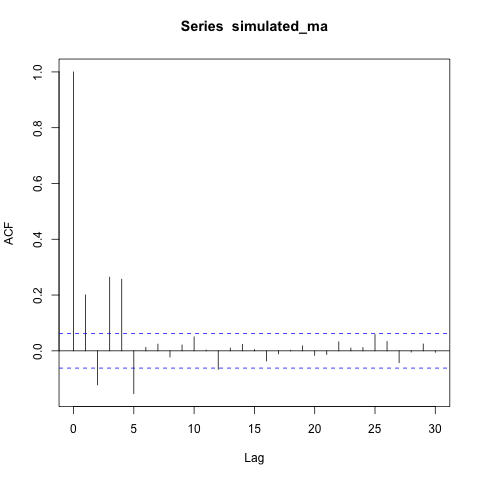
\includegraphics[width=2.5in]{acf-simulated-ma} 
   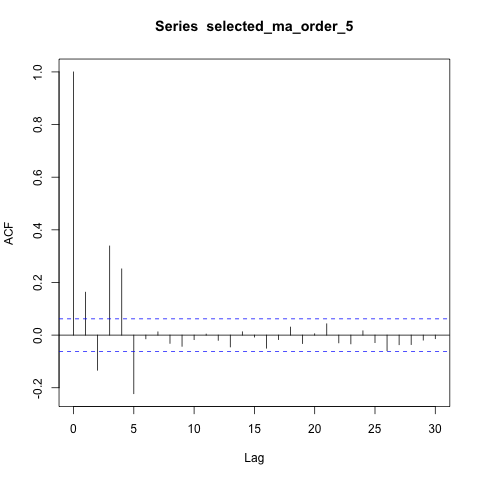
\includegraphics[width=2.5in]{acf-selected-ma} 
   \caption{Comparison of ACF of simulated MA(q) (left) and selected MA(5) (right)}
   \label{fig:acf}
\end{figure}

\begin{figure}[H] %  figure placement: here, top, bottom, or page
   \centering
   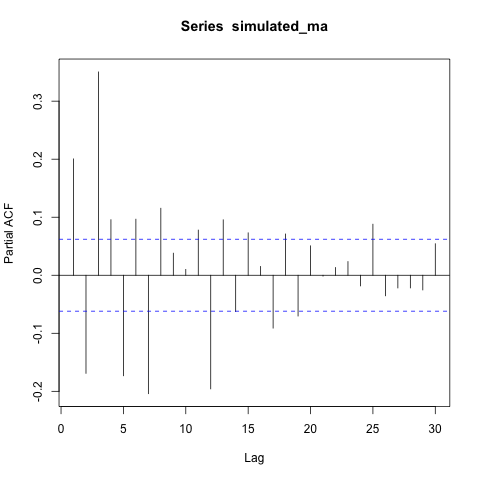
\includegraphics[width=2.5in]{pacf-simulated-ma} 
   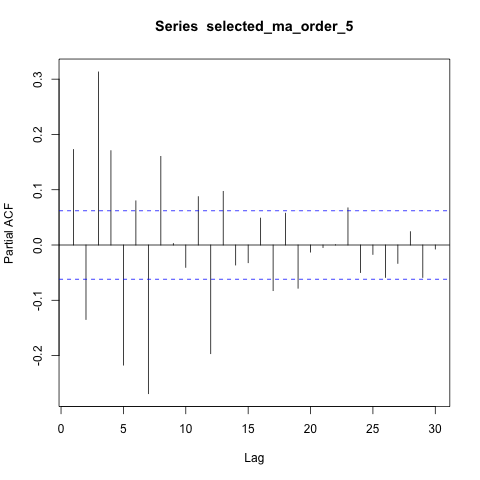
\includegraphics[width=2.5in]{pacf-selected-ma} 
   \caption{Comparison of PACF of simulated MA(q)(left) and selected MA(5) (right)}
   \label{fig:pacf}
\end{figure}
\justify
Figure \ref{fig:acf} and \ref{fig:pacf} shows the ACF and the PACF of the simulated MA(q) and a MA(5) where $q=5$ is selected from AIC and BIC penalty criteria.
We can observe that the simulated MA(q) is some what consistent with the selected MA(5) model.
%%%%%%%%%%%%%%%%%%%%%%%%%%%%%%%%%%%%%%%%%%%%%%%%%%%%%%%%%%%%%%%%%%%%%%%%%%%%%%%%%
\subsection{Part d}
We simulate an ARMA(2,2) of length $n=50$, with
\begin{equation}\label{eq:phi}
 \phi = (\phi_{1}=-0.7, \phi_{2}=0.2) 
 \end{equation}
 \begin{equation}\label{eq:theta}
 \theta = (\theta_{1}=0.3, \theta_{2}=-0.2)
 \end{equation}
 with 
 \begin{equation}
 N(0,4^{2}) \nonumber
 \end{equation}
 The process is simulated in R by 
 \begin{lstlisting}
arma2_2 <- arima.sim(n=50,list(ar=c(-0.7, 0.2),ma=c(0.3, -0.2)),sd=4)
\end{lstlisting}
which generate the following figure
\begin{figure}[H] %  figure placement: here, top, bottom, or page
   \centering
   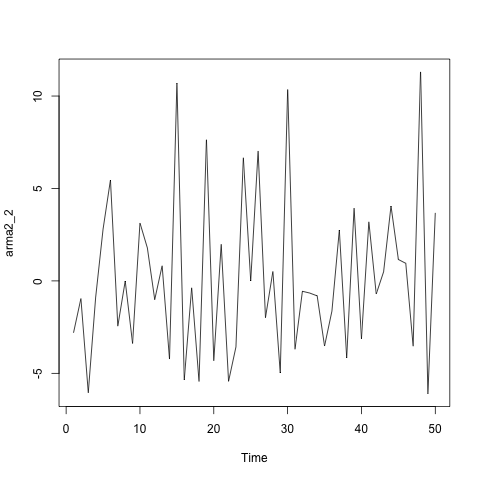
\includegraphics[width=4in]{simulated-arma2_2} 
   \caption{Simulated ARMA(2,2) with coefficients given by equation (\ref{eq:phi}) and (\ref{eq:theta}), with standard deviation 4}
   \label{fig:arma22}
\end{figure}
%%%%%%%%%%%%%%%%%%%%%%%%%%%%%%%%%%%%%%%%%%%%%%%%%%%%%%%%%%%%%%%%%%%%%%%%%%%%%%%%%%%%%%%%%%%%%%%%
\subsection{Part e}
Now we fit an ARMA(2,2) and a MA(5) from the simulated data from part d and use BIC and AIC criteria to select the optimum model.
\justify
Fit an ARMA(2,2) to the model
\begin{lstlisting}
arma2_2 <- arima.sim(n=50,list(ar=c(-0.7, 0.2),ma=c(0.3, -0.2)),sd=4)
fitted_ARMA_2_2_model <- arima(x=arma2_2,order=c(2,0,2), method="ML")
aic <- AIC(fitted_ARMA_2_2_model)
bic <- AIC(fitted_ARMA_2_2_model,k=log(length(fitted_ARMA_2_2_model)))
print(aic)
print(bic)

>295.4357
>299.2701
\end{lstlisting}
\justify
Fit a MA(5) process 

\begin{lstlisting}
arma2_2 <- arima.sim(n=50,list(ar=c(-0.7, 0.2),ma=c(0.3, -0.2)),sd=4)

fitted_MA5_model <- arima(x=arma2_2, order=c(0,0,5), method="ML")
aic <- AIC(fitted_MA5_model)
bic <- AIC(fitted_MA5_model,k=log(length(fitted_MA5_model)))
print(aic)
print(bic)

>286.4791
>290.9525
\end{lstlisting}
Since the BIC and AIC for the MA(5) process are the smallest we pick the MA(5) model
%%%%%%%%%%%%%%%%%%%%%%%%%%%%%%%%%%%%%%%%%%%%%%%%%%%%%%%%%%%%%%%%%%%%%%%%%%%%%%%%%%%%%%%%%%%%%%%
\subsection{Part f}
Now we repeat part e by increasing the sample size 500 times
\begin{figure}[H] %  figure placement: here, top, bottom, or page
   \centering
   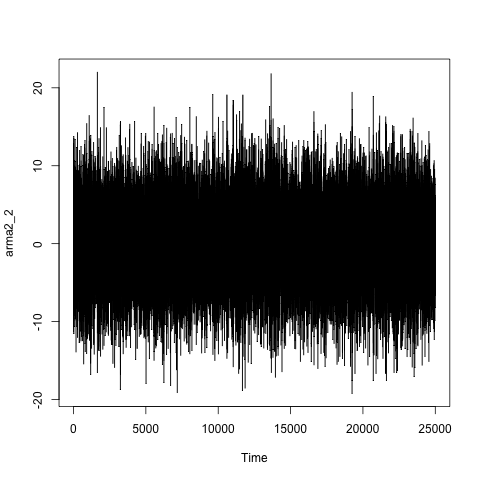
\includegraphics[width=4in]{simulated-arma2_2_plus} 
   \caption{Simulated ARMA(2,2) with sample size $50\times 500$}
   \label{fig:example}
\end{figure}
\justify
Fit an ARMA(2,2)
\begin{lstlisting}
arma2_2 <- arima.sim(n=50,list(ar=c(-0.7, 0.2),ma=c(0.3, -0.2)),sd=4)
fitted_ARMA_2_2_model <- arima(x=arma2_2,order=c(2,0,2), method="ML")
aic <- AIC(fitted_ARMA_2_2_model)
bic <- AIC(fitted_ARMA_2_2_model,k=log(length(fitted_ARMA_2_2_model)))
print(aic)
print(bic)

>142228.2
>142232.7
\end{lstlisting}
\justify
Fit a MA(5) process 

\begin{lstlisting}
arma2_2 <- arima.sim(n=50,list(ar=c(-0.7, 0.2),ma=c(0.3, -0.2)),sd=4)

fitted_MA5_model <- arima(x=arma2_2, order=c(0,0,5), method="ML")
aic <- AIC(fitted_MA5_model)
bic <- AIC(fitted_MA5_model,k=log(length(fitted_MA5_model)))
print(aic)
print(bic)

>142130
>142134.5
\end{lstlisting}
Again the MA(5) process comes with the lowest BIC and AIC and is the preferred model.

\section{Problem 9.2: Plotting basis function}
\begin{figure}[H] %  figure placement: here, top, bottom, or page
   \centering
   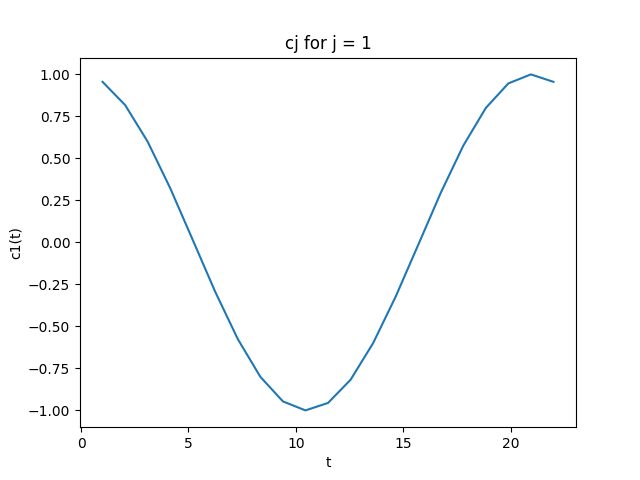
\includegraphics[width=2in]{cj1} 
    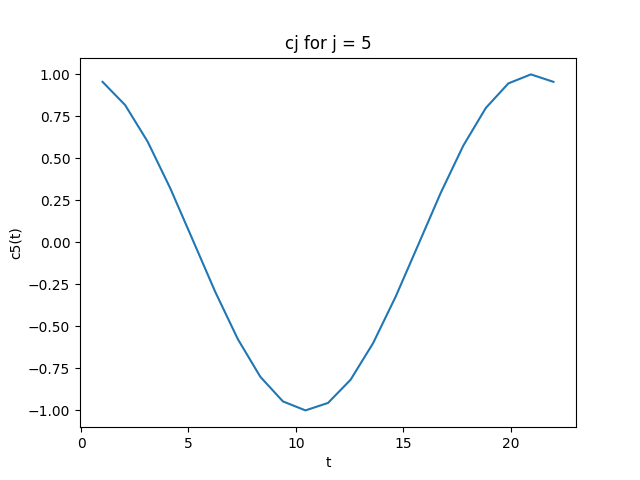
\includegraphics[width=2in]{cj5} 
     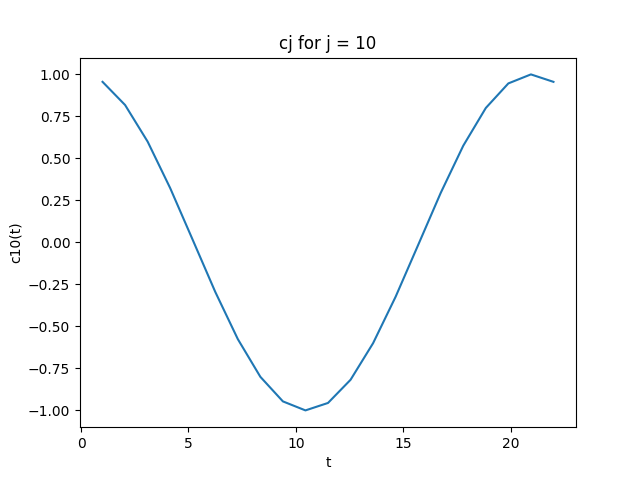
\includegraphics[width=2in]{cj10} 
   \caption{Plot of $c_{1}(t), c_{5}(t), c_{10}(t)$ on $t=[1,21]$}
   \label{fig:cj}
\end{figure}

\begin{figure}[H] %  figure placement: here, top, bottom, or page
   \centering
   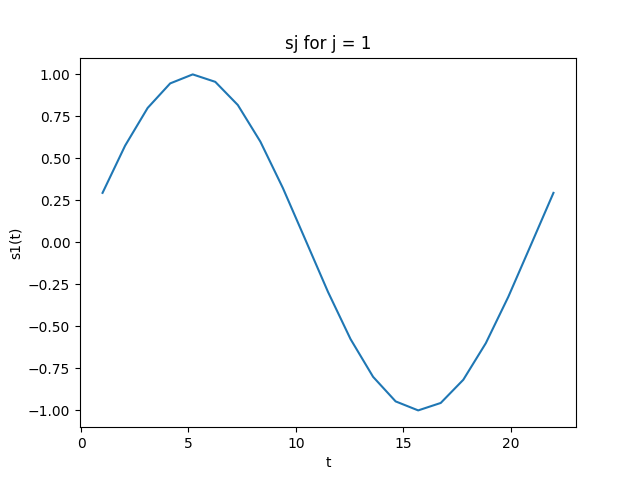
\includegraphics[width=2in]{sj1} 
    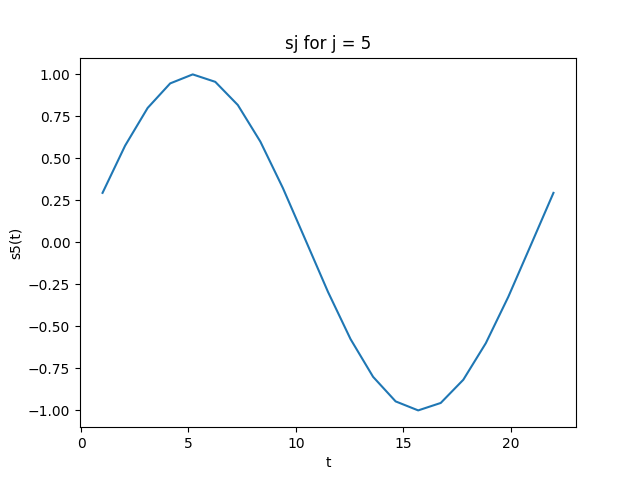
\includegraphics[width=2in]{sj5} 
     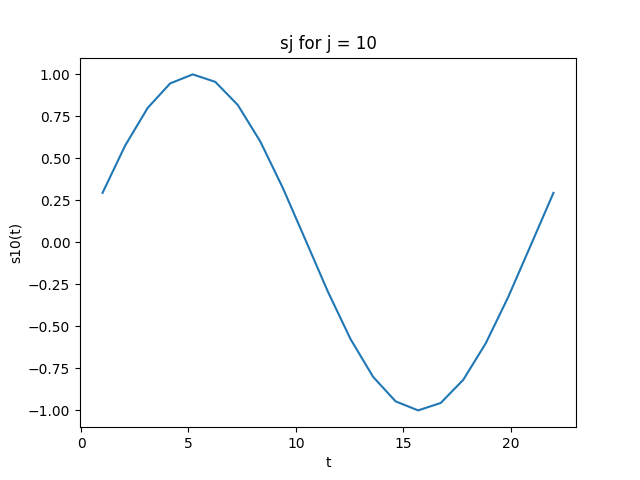
\includegraphics[width=2in]{sj10} 
   \caption{Plot of $s_{1}(t), s_{5}(t), _{10}(t)$ on $t=[1,21]$}
   \label{fig:sj}
\end{figure}

%%%%%%%%%%%%%%%%%%%%%%%%%%%%%%%%%%%%%%%%%%%%%%%%%%%%%%%%%%%%%%%%%%%%%%%%%%%%%%%%%%%%%%%%%%%%%
%%%%%%%%%%%%%%%%%%%%%%%%%%%%%%%%%%%%%%%%%%%%%%%%%%%%%%%%%%%%%%%%%%%%%%%%%%%%%%%%%%%%%%%%%%%%%

\section{Problem 9.3: White noise}
A white noise is a sequence of uncorrelated random variable $\{ X_{t} \}$, each with zero mean and finite variance $\sigma^{2}$ \cite{petter}. The white noise $\{ X_{t} \}$ is a stationary process with mean zero and covariance function given by \cite{petter}:
\begin{equation}
    \gamma_{X}(t+h,t)= 
\begin{cases}
    \sigma^{2},& \text{if } h=0\\
    0,              & \text{if } h \neq 0
\end{cases}
\end{equation}
If $\{ X_{t} \}$ is a white noise we write
\begin{equation}
\{ X_{t} \} \sim \textbf{WN}(0,\sigma^{2}).
\end{equation}
%
\section{Problem 9.4}
\subsection{Part a: simulation of an AR(2) process}
\begin{figure}[H] %  figure placement: here, top, bottom, or page
   \centering
   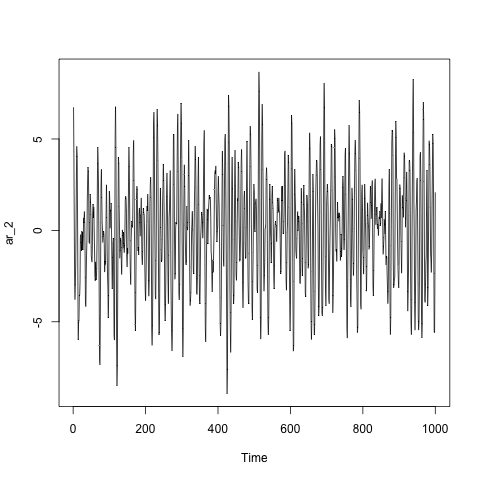
\includegraphics[width=4in]{p94ar2} 
   \caption{Simulation of the AR(2) process with $n=1000$, $\phi=(1.4, -0.8)$ and $\sigma^{2}=1$}
   \label{fig:example}
\end{figure}

%%%%%%%%%%%%%%%%%%%%%%%%%%%%%%%%%%%%%%%%%%%%%%%%%%%%%%%%%%

\subsection{Part b}
Let compute the matrix $G$ given by 
\begin{equation}
G = 
\begin{bmatrix}
    | & & | \\
    e_{-\left[ \frac{n-1}{2}\right]}&\cdots & e_{\left[ \frac{n}{2}\right]}\\
     | & & |\\
\end{bmatrix},
\end{equation}
where 

\begin{equation}
e_{k} = \frac{1}{\sqrt{n}}
\begin{bmatrix}
    e^{i\frac{2\pi k}{n}} \\
     e^{i\frac{4\pi k}{n}}\\
     \vdots \\
      e^{i2\pi k}
\end{bmatrix},
\end{equation}
So that 
\begin{equation}
\begin{split}
G &= \frac{1}{\sqrt{1000}}
\begin{bmatrix}
    | & & | \\
    e_{-\left[ \frac{n-1}{2}\right]}&\cdots & e_{\left[ \frac{n}{2}\right]}\\
     | & & |\\
\end{bmatrix}\\
&= \frac{1}{\sqrt{1000}}
\begin{bmatrix}
    e^{-i\frac{2\pi\times 499}{1000}} & \cdots& e^{i\pi} \\
     e^{-i\frac{4\pi\times 499}{1000}}&\cdots & e^{i2\pi}\\
     \vdots & \cdots & \vdots\\
      e^{-i499}& \cdots & e^{i5.10^{5}}\\
\end{bmatrix}\\
\end{split}
\end{equation}
\justify
And $a_{k}$ is given by 
\begin{equation}
a_{k} = \frac{1}{\sqrt{1000}}\sum_{t=1}^{1000}x_{t}e^{-it\frac{2\pi}{n}k}, \quad k=-499, \cdots 500
\end{equation}

%%%%%%%%%%%%%%%%%%%%%%%%%%%%%%%%%%%%%%%%%%%%%%%%%%%%%%%%%%%%%%%%%%%%%%%%%%%%%%%%%%%%%%%%%%%%%
%%%%%%%%%%%%%%%%%%%%%%%%%%%%%%%%%%%%%%%%%%%%%%%%%%%%%%%%%%%%%%%%%%%%%%%%%%%%%%%%%%%%%%%%%%%%%


\section{Problem 9.5}
We have 
\begin{equation}
g(\lambda) = K| a(e^{-i\lambda})  |^{2}, \quad K>0,
\end{equation}
where 
\begin{equation}
a(z) = 1+ \sum_{i=1}^{q}a_{i}z^{i}
\end{equation}
and g is strictly positive in $[-\pi, \pi]$
\subsection{Part a}
Suppose that the polynomial $a$ has root on the unit circle. Then $z=\pm1, \pm i$ are roots, meaning that
\begin{equation}
a(1) = 1+ \sum_{i=1}^{q}a_{i} = 0\Rightarrow \sum_{i=1}^{q}a_{i} = -1
\end{equation}
\begin{equation}
a(-1) = 1+ \sum_{i=1}^{q}a_{i}(-1)^{p} = 0\Rightarrow \sum_{i=1}^{q}a_{i}(-1)^{p} = -1
\end{equation}

\begin{equation}
a(i) = 1+ \sum_{i=1}^{q}a_{i}i^{p} = 0\Rightarrow \sum_{i=1}^{q}a_{i}i^{q} = -1
\end{equation}
\begin{equation}
a(-i) = 1+ \sum_{i=1}^{q}a_{i}(-i)^{p} = 0\Rightarrow \sum_{i=1}^{q}a_{i}(-i)^{p} = -1
\end{equation}

So we have 
\begin{equation}
\begin{split}
\sum_{i=1}^{q}a_{i} &=  \sum_{i=1}^{q}a_{i}i^{i}\\
\sum_{i=1}^{q}a_{i}-\sum_{i=1}^{q}a_{i}i^{i}&=0\\
\sum_{i=1}^{q}a_{i}(1-i^{q})&=0\\
a_{1}(1-i) + \cdots+ a_{q}(1-i^{q})&=0
\end{split}
\end{equation}
So that every coefficient with index of the sort $q=2^{r}$ where r is even will be zeros. If we repeat the same with they other equations, we see that all coefficient $a_{i} =0$ for 
$i = 1, \cdots, p$. This mean that 
\begin{equation}
a(z) = 1
\end{equation}
But if this is the case our assumption that a has root on the unit circle is not true, therefore a can not take root at the unit circle

\subsection{Part b}
By definition of invertible process, the polynomial a(B) does not have roots on the unit circle. We have shown that in part a.









\begin{thebibliography}{9}
\bibitem{ziak} 
John J. Dziak, Donna L. Coffman, Stephanie T. Lanza, Runze Li
\textit{Sensitivity and specificity of information criteria}. 
Addison-Wesley, Reading, Massachusetts, 1993.
 
\bibitem{petter} 
Petter J. Brockewell. Richard A. Davis 
\textit{Introduction to time series and forcasting}. 
Springer Text In Statistics, second edition
 \end{thebibliography}



\end{document}  